\documentclass{article}
\usepackage{graphicx} % Required for inserting images
\usepackage{pgfplots}
\pgfplotsset{compat=1.18}
\usepackage{float}
\usepackage{amsmath}
\usepackage{amssymb}

\title{Special Zealot Spawn Rates - Revealing the Truth}
%\author{}%
\date{August 2024}

\begin{document}

\maketitle

\section{Purpose}

There are still many misconceptions about the probability of Zealot kills per Special Zealot spawns that I want to clear up. There is a bit of math in this paper but you won't have to understand it to learn what I'm trying to say.

\section{Context}

Summoning Eyes have been a part of Hypixel Skyblock since August 2, 2019. The first rumor I heard about summoning eyes (back then) was that the chance of getting a summoning eye from a Zealot was $\frac{1}{5000}$. Obviously this rumor was quickly shown to be wrong. Initially, Special Zealots didn't exist and "normal" Zealots simply had a $\frac{1}{420}$ drop chance for a Summoning Eye. However, in SkyBlock Patch 0.7.3, they changed this to the Special Zealot system we currently have. In this patch, they also established the system where if the player takes multiple hits to kill a Zealot, they get a 10\% higher chance to summon a Special Zealot (which has at some point been changed to $11.\overline{1}$\%).

\vspace{2mm}

At certain kill thresholds, the player's Special Zealot spawn chance increases. Specifically, at 420, 630, and 840 Zealot kills when the player has not received an eye. Currently, the rates are $\frac{1}{210}$, $\frac{1}{140}$, and $\frac{1}{105}$, respectively, after reaching that point in Zealot kills without spawning a special Zealot.

\vspace{2mm}

Later down the line, the admins introduced the Zealot Bruiser, which had a base chance of $\frac{1}{380}$ to summon a Special Zealot. Similarly to (normal) Zealots, at certain kill thresholds, the chance to summon a Special Zealot increases. Specifically, at 380, 570, and 760 Zealot Bruiser kills from which the player has not summoned a Special Zealot, the odds increase to $\frac{1}{190}$, $\frac{1}{126.\overline{6}}$, and $\frac{1}{95}$ respectively.

\vspace{2mm}

There are multiple ways to increase special Zealot spawn rates. I will briefly list all of the methods:

\begin{enumerate}
    \item Max Zealuck increases your odds by \(1.\overline{1}\)x
    \item Taking Multiple Hits to kill Zealots/Zealot Bruisers increases your odds by \(1.\overline{1}\)x
    \item A Legendary or Mythic Enderman Pet increases your odds by \(1.25\)x
    \item Reaching Enderman Slayer 9 increases your odds by \(1.15\)x
\end{enumerate}

\vspace{2mm}

Note that not only does taking multiple hits to kill Zealots/Zealot Bruisers increase your odds of spawning a Special Zealot, but also decreases the amount of Zealot/Zealot Bruiser kills required to pass the kill thresholds.

\section{Math}

Firstly, we can use the expected value formula for a discrete random variable with parameters representing Special Zealot spawning probability:

\[
\sum_{i=1}^{n} x_i \cdot p(x_i) \rightarrow \sum_{x=1}^{\infty} x \cdot p(x)
\]

where for our first case (base probability, i.e. no increased odds) $x$ is the number of Zealots killed and $p(x)$ is the probability of acquiring a special Zealot at $x$th Zealot kill. Expanding $p(x)$ to its intervals produces

\[
p(x)_{min}, x \in \mathbb{Z} =
\begin{cases} 
\left(\frac{419}{420}\right)^{x-1} \cdot \frac{1}{420} & 1 \leq x \leq 420, \\
\left(\frac{419}{420}\right)^{420} \cdot \left(\frac{209}{210}\right)^{x-421} \cdot \frac{1}{210} & 421 \leq x \leq 630, \\
\left(\frac{419}{420}\right)^{420} \cdot \left(\frac{209}{210}\right)^{210} \cdot \left(\frac{139}{140}\right)^{x-631} \cdot \frac{1}{140} & 631 \leq x \leq 840, \\
\left(\frac{419}{420}\right)^{420} \cdot \left(\frac{209}{210}\right)^{210} \cdot \left(\frac{139}{140}\right)^{210} \cdot \left(\frac{104}{105}\right)^{x-841} \cdot \frac{1}{105} & x \geq 841.
\end{cases}
\]

The summations that model the expected value formula for a discrete random variable at the respective intervals associated with the probabilities above are

\[
E_1 = \sum_{n=1}^{420}\left(\left(\frac{419}{420}\right)^{n-1}\cdot\frac{n}{420}\right) = 111.35
\]

\vspace{3mm}

\[
E_2 = \sum_{n=421}^{630}\left(\left(\frac{419}{420}\right)^{420}\cdot\left(\frac{209}{210}\right)^{n-421}\cdot\frac{n}{210}\right) = 118.21
\]

\[
E_3 = \sum_{n=631}^{840}\left(\left(\frac{419}{420}\right)^{420}\cdot\left(\frac{209}{210}\right)^{210}\cdot\left(\frac{139}{140}\right)^{n-631}\cdot\frac{n}{140}\right) = 74.51
\]

\[
E_4 = \sum_{n=841}^{\infty}\left(\left(\frac{419}{420}\right)^{420}\cdot\left(\frac{209}{210}\right)^{210}\cdot\left(\frac{139}{140}\right)^{210}\cdot\left(\frac{104}{105}\right)^{n-841}\cdot\frac{n}{105}\right) = 28.28
\]

Now we can compute the average Zealots per Special Zealot:
\[
\sum_{x=1}^{\infty} x \cdot p(x) = \sum E_i = \text{ 111.35 + 118.21 + 74.51 + 28.28 = 332.35}
\]

Thus the average zealots per eye with base probability is 332.35! (Note that ``!''  is not being used as the factorial operator, but rather as an expression of excitement.)

\vspace{3mm}

\section{Graphs}

\begin{figure}[H]
\caption{Zealot Kill per Special Zealot with Base Probability}
\centering
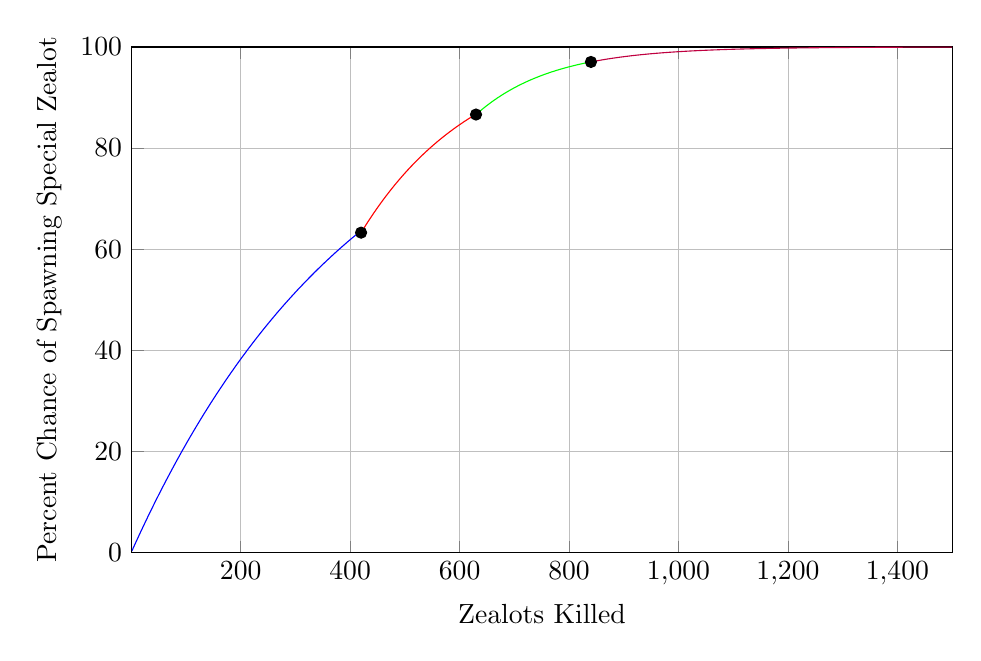
\begin{tikzpicture}
\begin{axis}[
    xlabel={Zealots Killed},
    ylabel={Percent Chance of Spawning Special Zealot},
    xmin=1, xmax=1500,
    ymin=0, ymax=100,
    grid=both,
    grid style={line width=.1pt, draw=gray!10},
    major grid style={line width=.2pt,draw=gray!50},
    width=12cm, height=8cm
]

\addplot [
    domain=1:420, 
    samples=100, 
    color=blue
]
{(1-(419/420)^x)*100};

\addplot [
    domain=420:630, 
    samples=100, 
    color=red
]
{(1-(209/210)^(x-420))*36.92 + 63.255};

\addplot [
    domain=630:841, 
    samples=100, 
    color=green
]
{(1-(139/140)^(x-630))*13.375 + 86.625};

\addplot [
    domain=841:1500, 
    samples=100, 
    color=purple
]
{(1-(139/140)^(x-840))*2.968 + 97.032};

\addplot[
    only marks,
    mark=*,
    mark options={scale=1,fill=black}
] coordinates {
    (420, 63.25589)
    (630, 86.62529)
    (840, 97.03166)
};

\end{axis}
\end{tikzpicture}
\end{figure}

Note the following:
\begin{enumerate}
    \item The percent chance never actually reaches 100\%
    \item The graph continues infinitely in the x-direction but is truncated to hide redundant information
\end{enumerate}


\end{document}


Now that we've calculated the average amount of Zealot kills per Special Zealot above, we can extend that to cases with increased odds. However, it's redundant to write out every possible combination of increased odds and the corresponding average Zealot kills per Special Zealot (if you'd like to using this computation procedure, go for it!) so instead I will only examine the case with the best possible odds.

This is when the player has max Zealuck (Tier 5), takes multiple hits to kill, is killing Zealot Bruisers, is using a Legendary or Mythic Enderman Pet, and has reached Enderman Slayer 9. Their probability intervals look like this:

\[
p(x)_{max}, x \in \mathbb{Z} =
\begin{cases} 
\left(\frac{419}{420}\right)^{x-1} \cdot \frac{1}{420} & 1 \leq x \leq 420, \\
\left(\frac{419}{420}\right)^{420} \cdot \left(\frac{209}{210}\right)^{x-421} \cdot \frac{1}{210} & 421 \leq x \leq 630, \\
\left(\frac{419}{420}\right)^{420} \cdot \left(\frac{209}{210}\right)^{210} \cdot \left(\frac{139}{140}\right)^{x-631} \cdot \frac{1}{140} & 631 \leq x \leq 840, \\
\left(\frac{419}{420}\right)^{420} \cdot \left(\frac{209}{210}\right)^{210} \cdot \left(\frac{139}{140}\right)^{210} \cdot \left(\frac{104}{105}\right)^{x-841} \cdot \frac{1}{105} & x \geq 841.
\end{cases}
\]
